\begin{question}{25}{
    De dreiging van verstoringen van onze kritieke infrastructuur op zee is een reeël en urgent probleem.
    De Nederlandse defensie wil deze dreiging het hoofd bieden door het inzetten van patrouilleschepen om spionageschepen van vijandelijke mogendheden
    te detecteren op een populaire vaarroute in de Noordzee.

    Uit historische data is de volgende kansfunctie op te maken voor het aantal te detecteren spionageschepen $X$ per dag:

    \begin{center}
        \begin{tabular}{cccccccc}
            \multicolumn{8}{c}{\textbf{Aantal spionageschepen per dag}} \\
            \toprule
                $k$ & $0$ & $1$ & $2$ & $3$ & $4$ & $5$ & $6$ \\
            \midrule
                $f(k) = P(X=k)$ & $0.06$ & $0.11$ & $0.17$ & $0.18$ & $0.22$ & $0.12$ & $0.14$ \\
            \bottomrule
        \end{tabular}
    \end{center}
}    
    \subquestion{4}{
        Teken het naalddiagram van deze discrete kansfunctie.
    }

    \solution{
        Het naalddiagram dat hoort bij deze kansfunctie ziet er als volgt uit:

        \begin{center}
            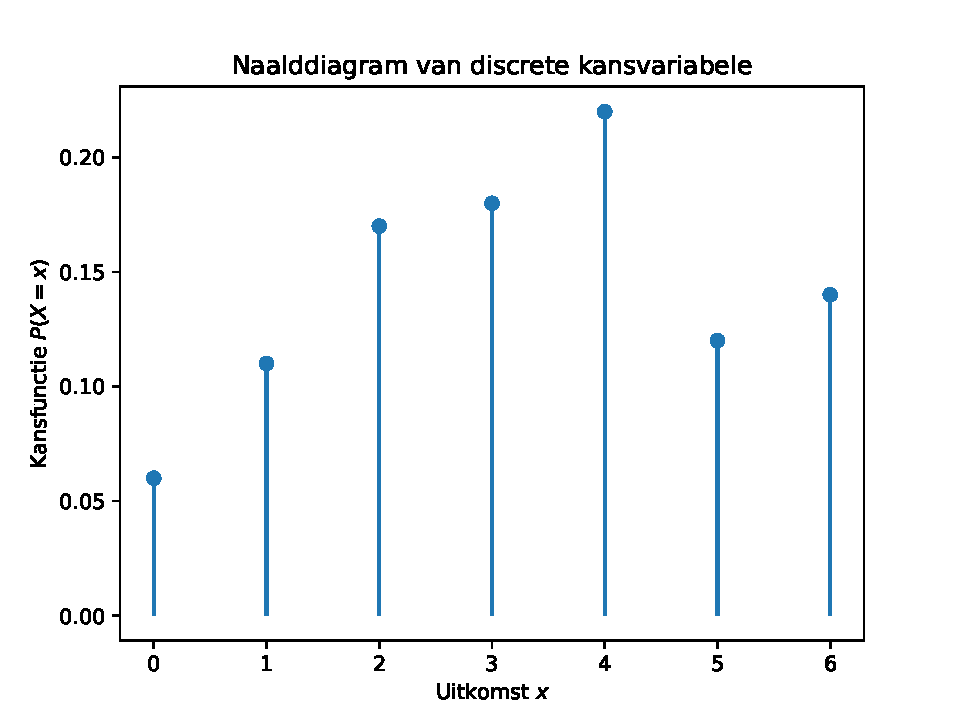
\includegraphics[width=0.9\textwidth]{../figures/exam20251017_1a.pdf} \rubric{4}
        \end{center}
    }

    \subquestion{4}{
        Toon aan dat deze kansfunctie inderdaad goed gedefinieerd is, dat wil zeggen, dat aan de twee voorwaarden van een kansfunctie wordt voldaan.
    }

    \solution{
        Een functie $f$ kan dienen als een kansfunctie als geldt:

        \textbf{Voorwaarde 1:} de functie $f$ is niet-negatief voor alle waarden van $k$, oftewel 
        \[
            f(k) \ge 0.
        \]
        Hier is voor alle mogelijke uitkomsten $k = 0, 1, \ldots, 6$ duidelijk aan voldaan. \rubric{2}

        \textbf{Voorwaarde 2:} de som van kansen over de uitkomstenruimte is gelijk aan 1, oftewel
        \[
            \sum_{k} f(k) = 1
        \]     
        
        Voor de tweede voorwaarde moeten we dus checken of de kansen op de uitkomsten $k = 0, 1, \ldots, 6$ sommeren tot 1.
        De som van kansen is gelijk aan
        \[
            \sum_{k} f(k) = 0.06 + 0.11 + 0.17 + 0.18 + 0.22 + 0.12 + 0.14 = 1
        \]
        Er is dus ook aan de tweede voorwaarde voldaan. Dit betekent dat de kansfunctie zoals beschreven in de tabel inderdaad goed gedefinieerd is.\rubric{2}
        
    }

    \subquestion{7}{
        Bereken de verwachtingswaarde $E[X]$ en de standaardafwijking $\sigma(X)$ van het aantal spionageschepen per dag.
    }
    \solution{
        De verwachtingswaarde $E[X]$ berekenen we door middel van
        \begin{align*}
            E[X] = \sum_k \cdot f(k)    &= \sum_{k=0}^6 k \cdot f(k) \\
                                        &= 0 \cdot 0.06 + 1 \cdot 0.11 + \ldots + 6 \cdot 0.14 \\
                                        &= 3.31 \rubric{2}          
        \end{align*}

        De standaardafwijking $\sigma(X)$ berekenen we door eerst de variantie $\Var{X}$ te bepalen, en van het resultaat de wortel te nemen:

        \begin{align*}
            \Var{X} = \sum_k (k - E[X])^2 \cdot f(k)    &= \sum_{k=0}^6 (k - 3.31)^2 \cdot f(k) \\
                                                        &= (0 - 3.31)^2 \cdot 0.06 + \ldots + (6 - 3.31)^2 \cdot 0.14 \\
                                                        &\approx 3.0139. \rubric{3}
        \end{align*} 
        \begin{align*}
             \Rightarrow \sigma(X) = \sqrt{\Var{X}} = \sqrt{3.0139} \approx 1.7361. \rubric{2}
        \end{align*}
    }

    \subquestion{3}{
        Bereken de kans dat er op een willekeurige dag minstens $4$ spionageschepen worden gedetecteerd.
    }

    \solution{
        Om de kans te berekenen dat er op een willekeurige dag minstens $4$ spionageschepen worden gedetecteerd, moeten we de kansen op tellen van uitkomsten groter dan of gelijk aan $4$. \rubric{1}
        Dit betekent dus:
        \begin{align*}
            P(X \ge 4) = P(X = 4) + P(X = 5) + P(X = 6) = 0.22 + 0.14 + 0.12 = 0.48. \rubric{1}
        \end{align*}
        Met kans $0.48$ worden minstens $4$ spionageschepen gedetecteerd. \rubric{1}
    }

    \subquestion{7}{
        Het probleem met spionageschepen is dat we aan het begin van de dag niet weten hoeveel spionageschepen er die dag zullen passeren.
        Voor ieder spionageschip geldt dat er minstens één patrouilleschip nodig is om het terug te begeleiden naar internationale wateren, maar het inzetten van een patrouilleschip is duur.
        Er wordt besloten om het aantal patrouilleschepen $Y$ per dag in te zetten volgens een binomiale verdeling met $n = 8$ en $p = 0.5$.
        Met hoeveel procent kans zijn er op een willekeurige dag voldoende patrouilleschepen aanwezig om alle spionageschepen die dag te kunnen detecteren en terug te begeleiden?     
    }

    \solution{
        Merk op dat er zodra er $k$ spionageschepen aanwezig zijn, dan kan ieder spionageschip terugbegeleid worden als er minstens $k$ patrouilleschepen zijn ingezet. \rubric{1}
        Dit betekent dat in het geval van $k$ spionageschepen, de kans dat alle schepen kunnen worden terugbegeleid gelijk is aan $P(Y \ge k)$.

        Gegeven is dat $Y$ binomiaal verdeeld is met $n = 8$ en $p = 0.5$.
        In andere woorden, deze kansen kunnen worden berekend met
        \begin{align*}
            P(Y \geq 0) &= 1 \\
            P(Y \geq 1) &= 1 - P(Y \leq 0) = 1 - \binomcdf(n=8, p=0.5, k=0) \approx 0.9961 \\
            P(Y \geq 2) &= 1 - P(Y \leq 1) = 1 - \binomcdf(n=8, p=0.5, k=1) \approx 0.9648 \\
            P(Y \geq 3) &= 1 - P(Y \leq 2) = 1 - \binomcdf(n=8, p=0.5, k=2) \approx 0.8555 \\
            P(Y \geq 4) &= 1 - P(Y \leq 3) = 1 - \binomcdf(n=8, p=0.5, k=3) \approx 0.6367 \\
            P(Y \geq 5) &= 1 - P(Y \leq 4) = 1 - \binomcdf(n=8, p=0.5, k=4) \approx 0.3633 \\
            P(Y \geq 6) &= 1 - P(Y \leq 5) = 1 - \binomcdf(n=8, p=0.5, k=5) \approx 0.1445 \rubric{3}
        \end{align*}
        Om nu de totale kans te berekenen dat er op een willekeurige dag voldoende patrouilleschepen zijn om alle spionageschepen die dag te kunnen detecteren en terug te begeleiden, moeten we ieder van deze uitkomsten vermenigvuldigen met de kans op dat betreffende aantal spionageschepen:
        \begin{align*}
            & P(X = 0) \cdot P(Y \ge 0) + P(X = 1) \cdot P(Y \ge 1) + \ldots + P(X = 6) \cdot P(Y \ge 6) \\
            & = 0.06 \cdot 1 + 0.11 \cdot 0.9961 + \ldots + 0.14 \cdot 0.1445 \\
            &= 0.6915 \rubric{2}
        \end{align*}     

        Met ruim $69$ procent kans zijn er voldoende patrouilleschepen aanwezig om alle spionageschepen terug te begeleiden naar internationale wateren. \rubric{1}

    }
\end{question}